\documentclass[11pt]{article}

\usepackage[utf8]{inputenc}
\usepackage[T1]{fontenc}
\usepackage[a4paper,margin=1in]{geometry}
\usepackage{graphicx}
\usepackage{booktabs}
\usepackage{longtable}
\usepackage{tabularx}
\usepackage{array}
\usepackage{float}
\usepackage{caption}
\usepackage{hyperref}
\usepackage{enumitem}
\usepackage{xcolor}

\setlength{\emergencystretch}{3em}
\setlist[itemize]{leftmargin=1.5em}
\setlist[enumerate]{leftmargin=1.5em}
\renewcommand{\arraystretch}{1.18}
\setcounter{tocdepth}{2}

\newcolumntype{Y}{>{\raggedright\arraybackslash}X}

\title{Technical Report on the Implemented \texttt{main} Corrosion Pipeline}
\author{Repository-grounded reconstruction from code, data files, saved artifacts, diagnostics, and local project documentation}
\date{\today}

\begin{document}

\maketitle

\begin{abstract}
This report reconstructs the \texttt{main} project strictly from its executable Python source, saved models, metric CSVs, cached image-feature table, the current raw workbook under \texttt{Data/}, and the thesis/conference PDFs stored in the repository documentation folders. The implemented system is not a single end-to-end image-to-RUL model. It is a three-task scikit-learn pipeline:
\begin{enumerate}
  \item \textbf{current\_corrosion}: predict the current label \texttt{B\_Peak\_Rust\_Percentage\_[\%]} from metadata plus handcrafted image features;
  \item \textbf{progression}: predict that same current corrosion label from metadata plus week only;
  \item \textbf{time\_to\_threshold}: predict a derived remaining-weeks target for specimens that eventually cross a fixed 20\% peak-rust threshold.
\end{enumerate}

The repository contains strong current-state evidence for visible corrosion quantification and weaker, more assumption-heavy evidence for metadata-driven progression and threshold timing. It also contains substantial reproducibility drift: the current raw workbook no longer matches the identifier and column conventions expected by the code, the image-feature cache is keyed by row-level IDs that the current loader no longer reconstructs, and the deployment manifest stores absolute artifact paths on another machine. This report therefore distinguishes carefully between what the saved artifacts support, what the present code still implements in principle, and what can no longer be rerun from the current raw files without repair.
\end{abstract}

\tableofcontents
\clearpage

\section{Problem framing}

\subsection{Actual problem solved by the implemented code}
The \texttt{main} repository implements a multi-model corrosion analytics workflow rather than a single direct predictor. The training script \texttt{main/train\_models.py} fits three separate supervised regression tasks:
\begin{itemize}
  \item \textbf{Task A: current corrosion}. Input is metadata plus handcrafted image features, and the target is the current observation's \texttt{B\_Peak\_Rust\_Percentage\_[\%]}.
  \item \textbf{Task B: progression}. Input is metadata plus \texttt{week}; the target is again the current observation's \texttt{B\_Peak\_Rust\_Percentage\_[\%]}. This is a metadata-conditioned regression of current corrosion against time, not a sequence model.
  \item \textbf{Task C: time to threshold}. Input is metadata, \texttt{week}, and \texttt{B\_Peak\_Rust\_Percentage\_[\%]}; the target is a derived value called \texttt{remaining\_weeks\_to\_threshold}, computed only for specimens that eventually cross a fixed threshold.
\end{itemize}

These three tasks share the same repository, but they are not equivalent scientifically. Task A is the closest to an image-based corrosion estimator. Task B is metadata-driven. Task C is a proxy timing model conditioned on current corrosion, not direct image-to-RUL learning.

\subsection{What is directly supervised and what is not}
The direct supervised quantities in \texttt{main} are:
\begin{itemize}
  \item \texttt{B\_Peak\_Rust\_Percentage\_[\%]} for Task A;
  \item \texttt{B\_Peak\_Rust\_Percentage\_[\%]} again for Task B;
  \item \texttt{remaining\_weeks\_to\_threshold} for Task C, but this target is derived inside the training script from the corrosion label and week, not read as a native raw column.
\end{itemize}

The following quantities are present in the current workbook but are not trained as targets in \texttt{main}:
\begin{itemize}
  \item \texttt{A\_Surface\_Total\_Rust\_Percentage[\%]}
  \item \texttt{A\_Total\_Rust\_Category\_(1--4)}
  \item \texttt{B\_Peak\_Rust\_Category\_(1--4)}
  \item \texttt{B\_Location\_of\_Peak\_Rus\_\ in\_length\_[cm]}
  \item \texttt{Last\_Wire\_Area\_Loss\_(Faliure\_Surface)\_\%}
  \item \texttt{Ultimate\_Load\_[kN]}
\end{itemize}

The structural labels are especially sparse in the current workbook: both wire-loss and ultimate-load values are non-null in only 48 rows, which corresponds to one terminal measurement per specimen.

\subsection{Why direct image-to-RUL is not supported}
Direct image-to-RUL is not implemented in this repository for four code-grounded reasons:
\begin{enumerate}
  \item No RUL column exists in the raw workbook or in the model interface.
  \item The only timing target is \texttt{remaining\_weeks\_to\_threshold}, which is created inside \texttt{train\_models.py} by finding the first week where \texttt{B\_Peak\_Rust\_Percentage\_[\%]} exceeds a fixed 20\% threshold.
  \item The time model is trained on \emph{true current corrosion labels}, not on image-derived predictions.
  \item The API also offers a second threshold-related mechanism: the progression endpoint sweeps week through the progression regressor and reports the first predicted crossing week. This is a heuristic threshold-crossing calculation, not an explicit survival or RUL model.
\end{enumerate}

\subsection{Exact scope of the implemented system}
The executable scope of \texttt{main} is:
\begin{itemize}
  \item parse the raw workbook into a feature table;
  \item derive specimen and time metadata from identifiers;
  \item compute or load handcrafted image features using fixed RGB thresholds and global color statistics;
  \item benchmark several tabular regressors under grouped specimen splits;
  \item save the best selected pipeline for each task;
  \item expose current corrosion, progression curve, and time-to-threshold inference through FastAPI.
\end{itemize}

It does \emph{not} implement:
\begin{itemize}
  \item direct sequence modeling from image streams;
  \item structural damage prediction from images;
  \item leave-one-treatment-out or leave-one-campaign-out evaluation;
  \item a single end-to-end image-to-threshold or image-to-RUL benchmark;
  \item monotonicity-constrained progression learning;
  \item censoring-aware survival analysis.
\end{itemize}

\section{Repository-grounded pipeline overview}

\subsection{Key repository components}

\begin{table}[H]
\centering
\small
\begin{tabularx}{\textwidth}{p{0.22\textwidth} p{0.73\textwidth}}
\toprule
\textbf{Component} & \textbf{Repository-grounded role} \\
\midrule
\texttt{main/data\_utils.py} & Raw workbook loading, numeric coercion, identifier parsing, derived temporal metadata, image-path construction, and dataset summary. \\
\texttt{main/image\_features.py} & Handcrafted image feature extraction using RGB threshold masks, RGB/HSV statistics, red-dominance features, and cache handling. \\
\texttt{main/modeling.py} & Candidate model definitions, preprocessing, grouped cross-validation, grouped holdout benchmarking, selection logic, and feature-importance extraction. \\
\texttt{main/train\_models.py} & Orchestrates all three tasks, saves metrics and feature importance tables, dumps the selected models, and writes the artifact manifest. \\
\texttt{main/inference.py} & Loads the saved manifest and model objects, assembles prediction rows, clips outputs, and implements progression and threshold inference logic. \\
\texttt{main/api.py} & FastAPI wrapper exposing \texttt{/health}, \texttt{/predict/current}, \texttt{/predict/progression}, and \texttt{/predict/time-to-threshold}. \\
\texttt{main/reports/*.csv} & Saved benchmark outputs: task-level metrics, feature-importance tables, and the cached image feature matrix. \\
\texttt{main/artifacts/*.joblib} and \texttt{manifest.json} & Saved production pipelines and metadata from the successful historical training run. \\
\bottomrule
\end{tabularx}
\caption{Executable repository components used to reconstruct the implemented system.}
\label{tab:repo_components}
\end{table}

\subsection{Pipeline stages}

\begin{table}[H]
\centering
\small
\begin{tabularx}{\textwidth}{p{0.13\textwidth} p{0.16\textwidth} p{0.16\textwidth} Y}
\toprule
\textbf{Stage} & \textbf{Input} & \textbf{Output} & \textbf{Purpose, design choice, and limitation} \\
\midrule
Data ingestion & Excel workbook + image directory & Raw dataframe with promoted semantic headers & \texttt{load\_corrosion\_dataframe()} assumes the first data row contains the semantic column names. This reflects the historical data snapshot but is brittle to workbook changes. \\
Dataset parsing & Raw dataframe & Derived \texttt{specimen}, \texttt{capture\_date}, \texttt{week}, \texttt{series}, \texttt{image\_path}, \texttt{image\_exists} & Designed to reconstruct row-level IDs and align each label row to an image. In the current raw workbook, this assumption is broken because \texttt{ID} is now specimen-level rather than row-level. \\
Image alignment / preprocessing & Existing PNG files & RGB arrays or cached features & No geometric alignment or segmentation pipeline is executed here. The code assumes preprocessed PNGs already exist and extracts global statistics and simple threshold masks only. \\
Image feature extraction & One image per row & 18 image features + corruption metadata & Uses fixed rust/black/gray RGB thresholds plus RGB/HSV summary statistics. Corrupted images are imputed by column median. \\
Feature-table assembly & Parsed dataframe + image feature table & \texttt{full\_df} & Merges on \texttt{ID}. This worked in the saved run but fails against the current workbook schema because cached image features are keyed by row-level IDs. \\
Task A benchmark & Metadata + image features & Current corrosion benchmark table and best pipeline & Predict current peak rust using grouped splitting by specimen. \\
Task B benchmark & Metadata + week & Progression benchmark table and best pipeline & Predict current peak rust as a function of metadata and week. This is not a sequence model and has no monotonicity constraint. \\
Task C proxy-threshold benchmark & Subset of specimens that cross 20\% peak rust & Time-to-threshold benchmark table and best pipeline & Derives a proxy timing target from the corrosion label. Excludes censored specimens entirely. \\
Artifact and report saving & Benchmarks + models & CSV metrics, feature importance tables, joblib pipelines, manifest & Saves aggregate outputs only. No per-row holdout predictions or specimen-level residual files are stored. \\
Inference / API & Metadata, image path, optional current corrosion input & Current corrosion, progression curve, or threshold timing response & Provides deployment wrappers, but the current manifest stores absolute paths on another machine, so loading currently fails locally. \\
\bottomrule
\end{tabularx}
\caption{Step-by-step reconstruction of the implemented pipeline and its main risks.}
\label{tab:pipeline_stages}
\end{table}

\subsection{Data ingestion and parsing details}
\paragraph{What the code expects.}
\texttt{main/data\_utils.py} expects:
\begin{itemize}
  \item row-level observation identifiers in the column named \texttt{ID}, formatted as \texttt{specimen-date-weekW};
  \item columns named \texttt{Ageing\_Days} and \texttt{NaCl\%};
  \item image files whose names are exactly \texttt{ID + ".png"}.
\end{itemize}

\paragraph{What the current workbook contains.}
The current workbook under \texttt{Data/Images\_Dataset\_A-Z.xlsx} has two leading semantic rows. After promoting the second row into headers, the available raw columns are \texttt{Sample Name}, \texttt{ID}, \texttt{N\_Steel\_Mesh}, \texttt{Treatment}, \texttt{Label\_Treatment}, \texttt{Ageing Days}, corrosion labels, cover, wire loss, and ultimate load. In this snapshot:
\begin{itemize}
  \item \texttt{Sample Name} holds row-level IDs such as \texttt{D01-20240110-0W};
  \item \texttt{ID} holds specimen IDs such as \texttt{D01};
  \item \texttt{Ageing Days} is spelled with a space, not an underscore;
  \item no direct raw column named \texttt{NaCl\%} is exposed.
\end{itemize}

\paragraph{Consequence.}
The historical training outputs are real, but the current code no longer parses the current raw workbook correctly. The parser now derives \texttt{week}, \texttt{specimen}, and \texttt{series} as all-missing, creates nonexistent image paths such as \texttt{D01.png}, and fails in \texttt{dataset\_summary()} before training proceeds.

\subsection{Image alignment and ID mapping}
No explicit alignment, registration, cropping, white-balance correction, or strip segmentation is executed in the code of \texttt{main}. Those operations are documented in the thesis and conference paper, but in this repository version they are treated as upstream preprocessing assumptions embodied in the existing PNG files and in the hand-coded RGB thresholds.

The only direct image-to-row mapping implemented in code is filename construction from \texttt{ID}. Because the current raw workbook now stores specimen IDs in that column, the live code maps rows to nonexistent files such as \texttt{Data/Images\_dataset/D01.png}. In the saved run, the row-level IDs still matched the image filenames, as evidenced by the 792-row image-feature cache.

\subsection{Cleaning and missing/corrupted-image handling}
Numeric columns are coerced with \texttt{pd.to\_numeric(errors="coerce")}. The scikit-learn preprocessors then apply median imputation to numeric features and most-frequent imputation to categorical ones.

Image corruption is handled inside \texttt{extract\_image\_features()}. If Pillow fails to open an image, every image feature is returned as \texttt{NaN}, the row is flagged as corrupted, and the full feature table later fills the numeric image columns with feature-wise medians.

In the saved artifacts there is exactly one corrupted image:
\begin{itemize}
  \item \texttt{E01-20240508-17W}
\end{itemize}

The current raw workbook contains 791 labeled rows, while \texttt{image\_features\_cache.csv} contains 792 IDs. The only cached ID not present in the current workbook is again \texttt{E01-20240508-17W}, so the corrupted row also coincides with the current data/artifact mismatch.

\subsection{Feature extraction}
The image branch is entirely handcrafted. \texttt{main/image\_features.py} creates:
\begin{itemize}
  \item RGB channel means: \texttt{img\_r\_mean}, \texttt{img\_g\_mean}, \texttt{img\_b\_mean};
  \item RGB channel standard deviations: \texttt{img\_r\_std}, \texttt{img\_g\_std}, \texttt{img\_b\_std};
  \item HSV channel means and standard deviations;
  \item \texttt{img\_rg\_diff\_mean};
  \item \texttt{img\_red\_dominance\_pct};
  \item \texttt{img\_rust\_mask\_pct}, \texttt{img\_black\_mask\_pct}, \texttt{img\_gray\_mask\_pct};
  \item \texttt{img\_rust\_to\_black\_ratio}.
\end{itemize}

The thresholds match the documented RGB ranges from the thesis and conference paper:
\begin{itemize}
  \item rust: \([25,0,0]\) to \([255,100,80]\);
  \item black pores: \([0,0,0]\) to \([5,5,0]\);
  \item gray/background: \([60,70,35]\) to \([120,105,95]\).
\end{itemize}

\subsection{Feature-family organization}
The model families used in training are:
\begin{itemize}
  \item metadata/context features: \texttt{N\_Steel\_Mesh}, \texttt{Treatment}, \texttt{NaCl\%}, \texttt{Ageing\_Days}, \texttt{Cover\_(Faliure\_Surface)\_[mm]}, \texttt{week}, \texttt{series};
  \item handcrafted image features: 18 global color and threshold-derived image variables;
  \item the derived threshold-timing input \texttt{B\_Peak\_Rust\_Percentage\_[\%]} for Task C.
\end{itemize}

There are no deep image embeddings, no morphology descriptors, no strip-wise image features, and no learned image backbone in this repository.

\subsection{Model training, evaluation, and proxy-RUL logic}
\texttt{main/modeling.py} benchmarks fixed candidate regressors under grouped splitting:
\begin{itemize}
  \item ElasticNet with \(\alpha=0.02\), \(l1\_ratio=0.2\), and \texttt{max\_iter=10000};
  \item RandomForestRegressor with 500 trees and \texttt{min\_samples\_leaf=2};
  \item GradientBoostingRegressor with default scikit-learn hyperparameters;
  \item optional XGBoost with 600 estimators, learning rate 0.03, depth 6, subsample 0.9, and \texttt{colsample\_bytree=0.8}.
\end{itemize}

Selection is heuristic, not tuned: the code sorts the benchmark table by \texttt{holdout\_mae}, then \texttt{cv\_mae}, then \texttt{holdout\_rmse}. The chosen model is then refit on the full dataset for production.

Proxy threshold logic appears in two places:
\begin{enumerate}
  \item Task C constructs \texttt{remaining\_weeks\_to\_threshold} from the first week a specimen reaches the threshold.
  \item The progression endpoint sweeps week through the progression regressor and returns the first predicted crossing week.
\end{enumerate}

These are repository-grounded threshold proxies, not direct survival or RUL models.

\section{Data description and data dictionary}

\subsection{Current raw data versus saved artifacts}

\begin{table}[H]
\centering
\small
\begin{tabularx}{\textwidth}{p{0.26\textwidth} p{0.13\textwidth} p{0.14\textwidth} Y}
\toprule
\textbf{Source} & \textbf{Rows} & \textbf{Specimens} & \textbf{Repository-grounded note} \\
\midrule
Current workbook after both semantic rows & 791 & 48 & The current raw workbook exposes row-level identifiers in \texttt{Sample Name}, not in \texttt{ID}. \\
Current image directory & 792 PNGs & 48 & Includes the corrupted image \texttt{E01-20240508-17W.png}. \\
Saved image-feature cache & 792 cached IDs & 48 & One cached row has no counterpart in the current workbook: \texttt{E01-20240508-17W}. \\
Saved manifest and metric CSVs & 792 training rows reported & 48 & Evidence that the historical training run used a data snapshot with 792 aligned rows. \\
\bottomrule
\end{tabularx}
\caption{The current raw files and the saved training artifacts no longer describe exactly the same dataset snapshot.}
\label{tab:raw_vs_artifact}
\end{table}

\subsection{Code-workbook mismatches that matter for reproducibility}

\begin{table}[H]
\centering
\small
\begin{tabularx}{\textwidth}{p{0.27\textwidth} p{0.28\textwidth} Y}
\toprule
\textbf{Code expectation} & \textbf{Current raw workbook reality} & \textbf{Consequence} \\
\midrule
\texttt{ID} contains row-level strings like \texttt{D01-20240110-0W} & \texttt{ID} now contains specimen IDs like \texttt{D01}; row-level IDs are in \texttt{Sample Name} & Parsed \texttt{specimen}, \texttt{week}, \texttt{series}, and \texttt{image\_path} are wrong in live code. \\
\texttt{Ageing\_Days} exists & Current workbook column is \texttt{Ageing Days} & Feature selection by code no longer matches raw columns. \\
\texttt{NaCl\%} exists as a raw column & No direct \texttt{NaCl\%} column is exposed in the current workbook & The raw provenance of this trained feature cannot be reconstructed from the current workbook alone. \\
\texttt{B\_Peak\_Rust\_Category\_(1--5)} constant in code & Current workbook column is \texttt{B\_Peak\_Rust\_Category\_(1--4)} & Minor schema mismatch; the category constant is unused, but it signals repository drift. \\
Image files named from \texttt{ID} & Live code now constructs nonexistent files such as \texttt{D01.png} & \texttt{image\_exists} is false for all 791 current rows. \\
Image-feature cache merges on \texttt{ID} & Cache is keyed by row-level IDs, but the live dataframe now contains specimen IDs & Cached image features no longer align and become all-\texttt{NaN} when merged in the current repository state. \\
\bottomrule
\end{tabularx}
\caption{Current code-data mismatches that prevent exact reruns from the present raw snapshot.}
\label{tab:code_data_mismatch}
\end{table}

\subsection{Metadata dictionary}

\begin{longtable}{p{0.24\textwidth} p{0.18\textwidth} p{0.16\textwidth} p{0.13\textwidth} p{0.21\textwidth}}
\toprule
\textbf{Variable} & \textbf{Meaning / unit} & \textbf{Source} & \textbf{Role} & \textbf{Repository-grounded note} \\
\midrule
\endfirsthead
\toprule
\textbf{Variable} & \textbf{Meaning / unit} & \textbf{Source} & \textbf{Role} & \textbf{Repository-grounded note} \\
\midrule
\endhead
\texttt{Sample Name} & Row-level observation ID & Current workbook & Original identifier & Holds strings of the form \texttt{specimen-date-weekW}. Not used by live code, though it now carries the correct row key. \\
\texttt{ID} & Specimen identifier & Current workbook & Original metadata & Current live code treats this as if it were still the row-level ID. \\
\texttt{specimen} & Specimen/material identifier & Derived in code & Grouping variable & In the live code this is currently all-missing because the regex is applied to specimen IDs rather than row IDs. \\
\texttt{capture\_date} & Observation date & Derived in code & Temporal metadata & Derived only when the row-level ID is parsed correctly. \\
\texttt{week} & Observation week number & Derived in code / recoverable from \texttt{Sample Name} & Feature and grouping context & In the current workbook, exact \texttt{week} can still be recovered from \texttt{Sample Name}. \\
\texttt{Ageing Days} & Exposure duration in days & Current workbook & Original metadata & In the current workbook it satisfies \(\texttt{Ageing Days} = 7 \times \texttt{week}\) exactly. \\
\texttt{Ageing\_Days} & Exposure duration in days & Expected by code and manifest & Intended feature & Feature name used during historical training; currently absent under that exact raw column name. \\
\texttt{Treatment} & Treatment code & Current workbook & Metadata / categorical feature & Values in current raw data are \{MI, NO, PA, SA, SA\_PA, SA\_VF, VF\}. \\
\texttt{Label\_Treatment} & Additional treatment-family label & Current workbook & Metadata, unused & Values are \{D, G, MI, SA, VF\}; exact semantic mapping is not documented in the code. \\
\texttt{N\_Steel\_Mesh} & Number of mesh layers & Current workbook & Metadata / numeric feature & Used in all three trained tasks. \\
\texttt{Cover\_(Faliure\_Surface)\_[mm]} & Cover thickness on failure surface, mm & Current workbook & Metadata / numeric feature & Used in all three tasks and highly important in the progression model. \\
\texttt{NaCl\%} & Salt concentration & Expected by code and manifest & Intended numeric feature & Present in historical training features but not directly exposed in the current workbook; provenance currently ambiguous. \\
\texttt{series} & Alphabetic family from specimen prefix & Derived in code & Metadata / categorical feature & Serves as a family or campaign surrogate. The code contains no explicit raw campaign column. \\
\texttt{image\_path} & Path to PNG file & Derived in code & Alignment field & Correct only when row-level IDs are available in the parsed identifier column. \\
\texttt{image\_exists} & Whether the PNG path exists & Derived in code & Data-quality flag & In the current live parse it is false for all rows because the filenames are wrong. \\
\bottomrule
\caption{Metadata and identifier fields relevant to the \texttt{main} pipeline.}
\label{tab:metadata_dictionary}
\end{longtable}

\subsection{Labels, targets, and derived targets}

\begin{longtable}{p{0.26\textwidth} p{0.17\textwidth} p{0.11\textwidth} p{0.12\textwidth} p{0.22\textwidth}}
\toprule
\textbf{Variable} & \textbf{Meaning / unit} & \textbf{Density} & \textbf{Role} & \textbf{Repository-grounded note} \\
\midrule
\endfirsthead
\toprule
\textbf{Variable} & \textbf{Meaning / unit} & \textbf{Density} & \textbf{Role} & \textbf{Repository-grounded note} \\
\midrule
\endhead
\texttt{A\_Surface\_Total\_Rust\_Percentage[\%]} & Total surface rust percentage & 791/791 & Original corrosion label, unused target & Dense label. In the current workbook it correlates with \texttt{B\_Peak\_Rust\_Percentage\_[\%]} at 0.9495. \\
\texttt{A\_Total\_Rust\_Category\_(1--4)} & Surface-rust category & 791/791 & Unused label & Present but not modeled. \\
\texttt{B\_Peak\_Rust\_Percentage\_[\%]} & Peak local rust percentage & 791/791 current raw; 792/792 saved artifacts & \textbf{Primary direct target} & Used as the direct regression target in Tasks A and B, and as an input to Task C. \\
\texttt{B\_Peak\_Rust\_Category\_(1--4)} & Peak-rust category & 791/791 & Unused label & Current workbook uses a 1--4 coding, while a 1--5 constant exists unused in code. \\
\texttt{B\_Location\_of\_Peak\_Rus\_\ in\_length\_[cm]} & Location of the peak rust along the specimen, cm & 791/791 & Unused label & Not used in training or inference. \\
\texttt{Last\_Wire\_Area\_Loss\_(Faliure\_Surface)\_\%} & Terminal wire area loss & 48/791 & Structural endpoint, unused & One non-null value per specimen only. Values lie in \([0,0.5698]\) despite the percent suffix, so the stored unit may be fraction-like rather than percentage points. \\
\texttt{Ultimate\_Load\_[kN]} & Terminal ultimate load, kN & 48/791 & Structural endpoint, unused & One non-null value per specimen only. Range in the current workbook is 1.60--2.87 kN. \\
\texttt{remaining\_weeks\_to\_threshold} & Weeks remaining until first \(20\%\) peak-rust crossing & Derived inside \texttt{train\_models.py} & \textbf{Proxy timing target} & Created only for specimens that actually cross the threshold. Not available as a raw label. \\
\bottomrule
\caption{Label fields in the raw workbook and their actual role in the implemented system.}
\label{tab:label_dictionary}
\end{longtable}

\subsection{Dense versus sparse labels}

\begin{figure}[H]
\centering
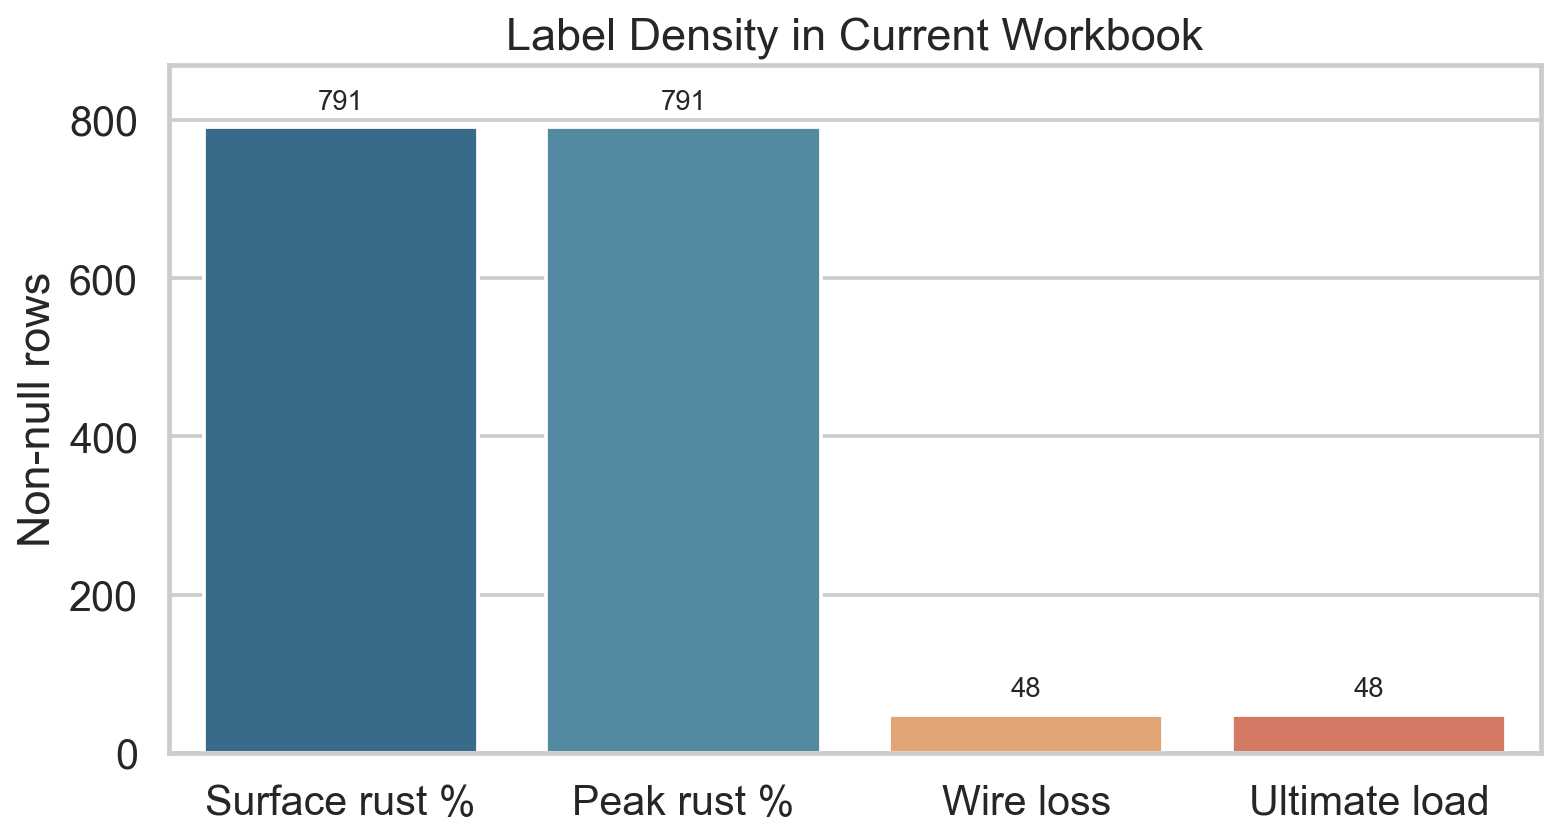
\includegraphics[width=0.78\textwidth]{reports/fig_label_density.png}
\caption{Non-null label counts in the current workbook. Surface and peak rust are dense row-level labels; wire loss and ultimate load are sparse terminal labels, available once per specimen.}
\label{fig:label_density}
\end{figure}

Figure~\ref{fig:label_density} shows why direct structural-damage modeling is not supported in \texttt{main}: the corrosion labels are dense, but the structural labels are terminal and sparse.

\section{Feature engineering}

\subsection{Implemented image-derived features}

\begin{table}[H]
\centering
\small
\begin{tabularx}{\textwidth}{p{0.22\textwidth} p{0.25\textwidth} Y Y}
\toprule
\textbf{Feature family} & \textbf{Implemented variables} & \textbf{Physical meaning and likely correlation} & \textbf{Weaknesses and risks} \\
\midrule
Global RGB statistics & \texttt{img\_r/g/b\_mean}, \texttt{img\_r/g/b\_std} & Capture average channel brightness and color spread; may respond to rust staining, lighting, and surface background. & Sensitive to illumination and preprocessing drift; not localized; can absorb acquisition bias. \\
Global HSV statistics & \texttt{img\_h/s/v\_mean}, \texttt{img\_h/s/v\_std} & Approximate hue, saturation, and brightness distributions; rust tends to alter hue and saturation. & Also global and non-localized; sensitive to white-balance mismatch. \\
Relative redness & \texttt{img\_rg\_diff\_mean}, \texttt{img\_red\_dominance\_pct} & Measures how strongly red channel exceeds green; likely associated with rust-colored staining. & Strong shortcut risk when the target itself is defined from rust-colored surface evidence. \\
Threshold masks & \texttt{img\_rust\_mask\_pct}, \texttt{img\_black\_mask\_pct}, \texttt{img\_gray\_mask\_pct} & Estimates global fractions of rust-like, pore-like, and gray/background-like pixels using thesis-matched RGB thresholds. & High tautology risk: the feature engineering reuses a threshold logic close to the documented label-generation pipeline. Still global, not strip-based. \\
Normalized ratio & \texttt{img\_rust\_to\_black\_ratio} & Rust-like area relative to pore-like area. Intended to normalize rust evidence by dark background/void prevalence. & Unstable when black-mask proportion is tiny; denominator protected only by \(10^{-6}\). \\
\bottomrule
\end{tabularx}
\caption{Actual image-derived features implemented in \texttt{main}.}
\label{tab:image_feature_families}
\end{table}

\subsection{What is not implemented}
The \texttt{main} repository does \emph{not} implement:
\begin{itemize}
  \item strip-wise corrosion features;
  \item morphology descriptors;
  \item connected-component counts;
  \item texture features such as GLCM or LBP;
  \item deep CNN embeddings;
  \item learned segmentation masks;
  \item brightness normalization beyond whatever is already present in the upstream PNG images.
\end{itemize}

This matters because the thesis and conference documentation describe strip-based or class-based workflows that are richer than the compact global descriptors used here.

\subsection{Feature families used by each model}

\begin{table}[H]
\centering
\small
\begin{tabularx}{\textwidth}{p{0.18\textwidth} p{0.18\textwidth} Y Y}
\toprule
\textbf{Task} & \textbf{Feature count} & \textbf{Feature set} & \textbf{Interpretation} \\
\midrule
Current corrosion & 25 & 7 base metadata features + 18 image features & Mixed model, but the saved feature importance shows it is overwhelmingly driven by the rust-mask feature. \\
Progression & 7 & Metadata only: mesh, treatment, intended saline, ageing days, cover, week, series & Purely metadata-driven conditional corrosion regression; not image-driven and not sequence-aware. \\
Time to threshold & 8 & Base metadata + \texttt{B\_Peak\_Rust\_Percentage\_[\%]} & Proxy timing model conditioned heavily on current true corrosion and week. \\
\bottomrule
\end{tabularx}
\caption{Feature sets used by the three trained tasks.}
\label{tab:task_feature_sets}
\end{table}

\subsection{Feature dominance and tautology risk}

\begin{figure}[H]
\centering
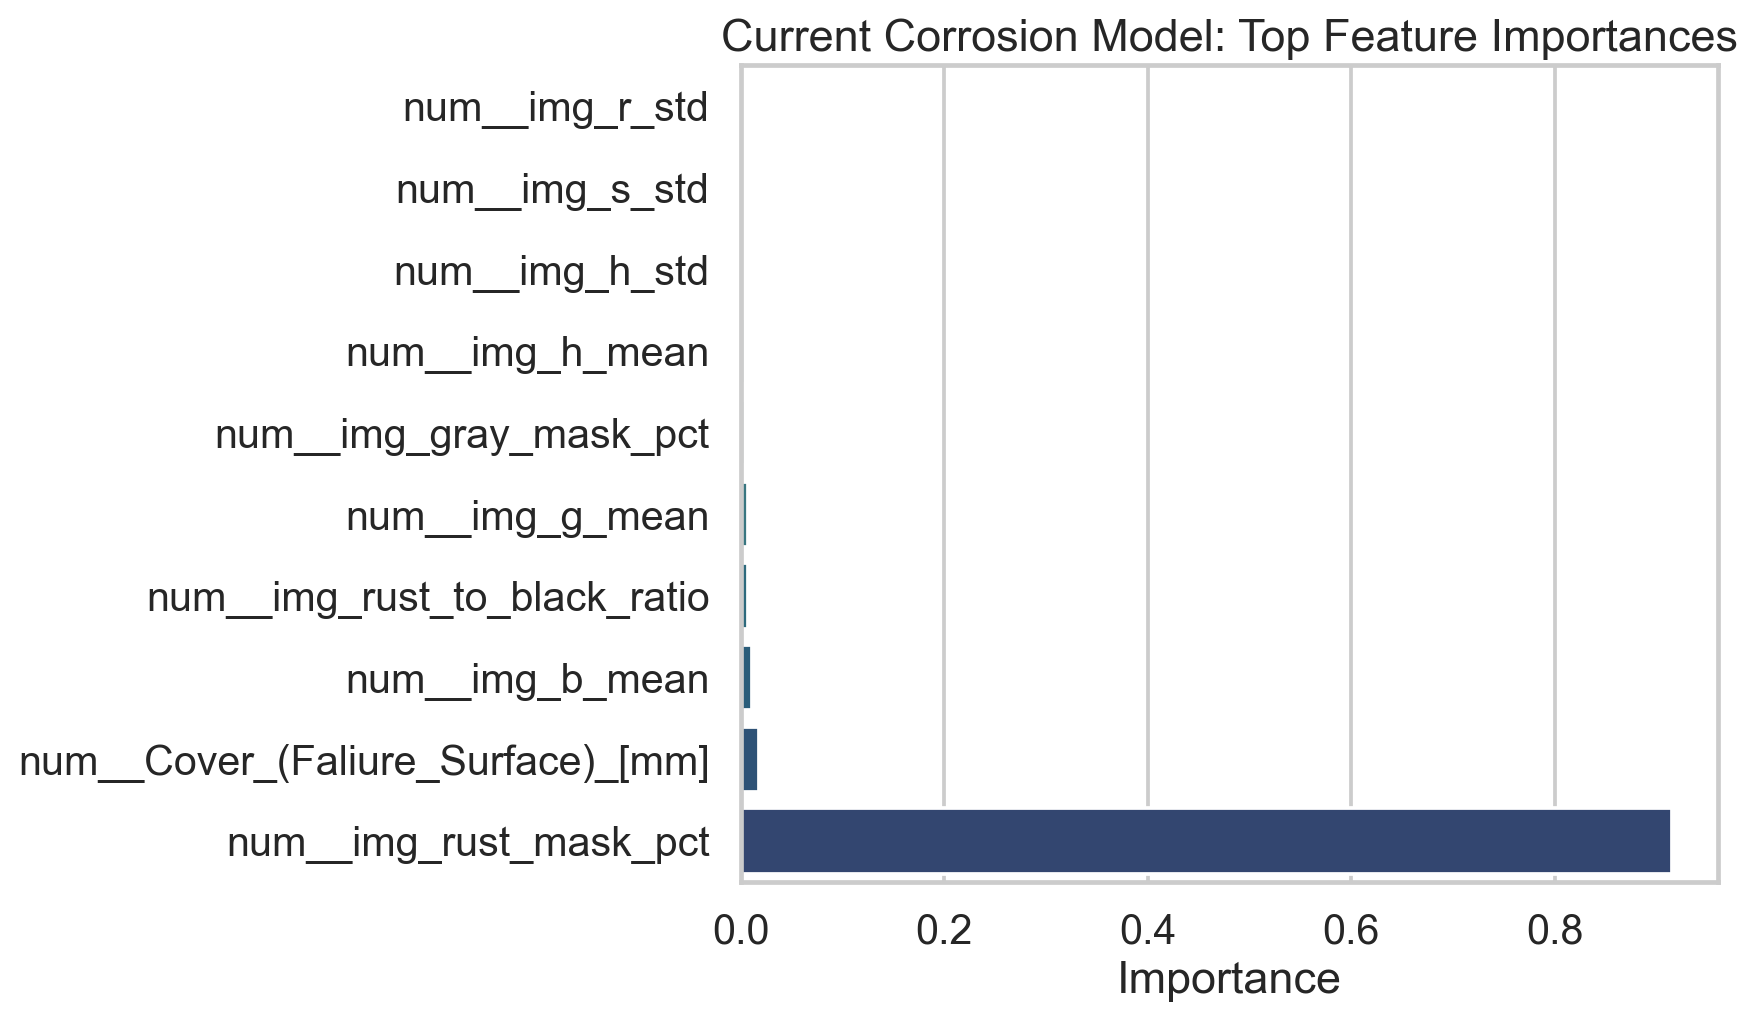
\includegraphics[width=0.82\textwidth]{reports/fig_current_feature_importance.png}
\caption{Top feature importances for the selected current-corrosion model. The handcrafted rust-mask percentage dominates the model.}
\label{fig:current_importance}
\end{figure}

The saved \texttt{current\_corrosion} feature-importance table shows that \texttt{img\_rust\_mask\_pct} alone contributes 0.915 of the total RandomForest importance. The top two features (\texttt{img\_rust\_mask\_pct} and cover thickness) sum to 0.933, and the top five sum to 0.958.

This is scientifically important:
\begin{itemize}
  \item The handcrafted rust-mask percentage uses the same rust RGB threshold family described in the thesis and conference paper.
  \item When the cached image features are joined back to the current workbook by row-level identifier, \texttt{img\_rust\_mask\_pct} correlates with \texttt{B\_Peak\_Rust\_Percentage\_[\%]} at 0.9495.
  \item The current-corrosion model is therefore highly interpretable, but it is also partly reconstructive: it is learning from a handcrafted visual quantity that is very close to the visible rust label.
\end{itemize}

\subsection{Redundancy, instability, and campaign dependence}
Three concrete risks appear in the implemented features:
\begin{enumerate}
  \item \textbf{Temporal duplication.} In the current workbook, \texttt{Ageing Days} equals \(7 \times \texttt{week}\) exactly. Yet the code trains on both \texttt{Ageing\_Days} and \texttt{week}, producing perfect temporal redundancy.
  \item \textbf{Family dependence.} \texttt{series}, cover thickness, treatment, and intended saline condition encode specimen-family structure. These are not purely corrosion descriptors.
  \item \textbf{Inference inconsistency.} The progression and time-to-threshold APIs ask the user for both \texttt{week} and \texttt{ageing\_days}. The README examples hold \texttt{ageing\_days=260} while varying or using weeks such as 22 or 28, even though the current raw data satisfy \(\texttt{Ageing Days} = 7 \times \texttt{week}\). That means the documented API usage is out-of-distribution relative to the current raw data.
\end{enumerate}

\section{Technical challenges and implemented responses}

\begin{longtable}{p{0.20\textwidth} p{0.25\textwidth} p{0.20\textwidth} p{0.25\textwidth}}
\toprule
\textbf{Challenge} & \textbf{How it was detected} & \textbf{Implemented handling} & \textbf{Residual risk} \\
\midrule
\endfirsthead
\toprule
\textbf{Challenge} & \textbf{How it was detected} & \textbf{Implemented handling} & \textbf{Residual risk} \\
\midrule
\endhead
Workbook schema drift & Current raw workbook now uses \texttt{Sample Name}, \texttt{Ageing Days}, and specimen-level \texttt{ID}. & None in live code. Historical artifacts still exist. & Fresh training now fails before benchmarking, so the repository is not currently reproducible end to end. \\
Image-ID misalignment & Live code constructs \texttt{D01.png}-style paths; all 791 current \texttt{image\_exists} flags become false. & None in live code. The saved image-feature cache preserves the historical aligned IDs. & Even cached features no longer merge because the current live dataframe uses the wrong IDs. \\
Corrupted image file & \texttt{image\_features\_cache.csv} and \texttt{manifest.json} both record \texttt{E01-20240508-17W} as corrupted. & Median-impute the image features. & The corrupted row is also the row missing from the current workbook, so exact raw/artifact alignment is uncertain. \\
Sparse structural supervision & Current workbook has only 48 non-null wire-loss rows and 48 non-null ultimate-load rows. & No structural model is trained in \texttt{main}. & Any structural or hidden-damage claim would exceed the evidence. \\
Repeated-measures leakage risk & Each specimen has 15, 17, or 18 observations across time. & Group-aware holdout split and GroupKFold by specimen. & Leakage by exact specimen is controlled, but no stricter treatment/campaign transfer tests are implemented. \\
Metadata shortcut learning & Progression and time models rely entirely or primarily on metadata and current corrosion values. & None beyond grouped splitting. & Strong current performance may not imply physically robust transfer. \\
Perfect temporal redundancy & In the current workbook \texttt{Ageing Days} equals \(7 \times \texttt{week}\) exactly. & None; both are still used as separate features in code. & Redundant timing inputs can distort feature-importance interpretation and create inconsistent API usage. \\
Holdout-based model selection & \texttt{evaluate\_models()} sorts by holdout MAE, then refits the selected model on the full dataset. & None. & The chosen production model is selected using the same holdout metrics later reported, and the final saved artifact is not the exact pipeline used to produce those holdout scores. \\
Path portability & \texttt{manifest.json} stores absolute paths under \texttt{/Users/youseffayyaz/...}. & None. & \texttt{load\_artifacts()} fails locally even though the local joblib files exist. \\
Documentation mismatch & README and \texttt{scientific\_solution.txt} imply deployable status and show temporally inconsistent examples. & None. & User-facing documentation overstates current reproducibility and blurs the distinction between proxy timing and direct RUL. \\
\bottomrule
\caption{Real implementation challenges and their remaining risks.}
\label{tab:challenges}
\end{longtable}

\section{Modeling methodology}

\subsection{Shared preprocessing and evaluation logic}
All three tasks use the same general scikit-learn design:
\begin{itemize}
  \item numeric features: median imputation + standardization;
  \item categorical features: most-frequent imputation + one-hot encoding with unknown-category tolerance;
  \item a single grouped holdout split generated by \texttt{GroupShuffleSplit(test\_size=0.2, random\_state=42)};
  \item grouped cross-validation on the training portion using \texttt{GroupKFold} with up to 5 folds;
  \item candidate models ranked by \texttt{holdout\_mae}, then \texttt{cv\_mae}, then \texttt{holdout\_rmse}.
\end{itemize}

No grid search, random search, repeated holdout, or uncertainty quantification is implemented.

\subsection{Task A: current corrosion}
\paragraph{Target.}
\texttt{B\_Peak\_Rust\_Percentage\_[\%]}.

\paragraph{Feature set.}
7 base metadata fields plus 18 handcrafted image features.

\paragraph{Best selected model and interpretation.}
RandomForest was selected by holdout MAE. The saved holdout MAE is 2.3794, RMSE 4.2543, and \(R^2=0.8996\). This is the strongest result in the repository, but it must be interpreted as visible corrosion quantification, not hidden-damage inference.

\paragraph{What the model can and cannot learn.}
Because the dominant signal is \texttt{img\_rust\_mask\_pct}, the model can learn current visible rust evidence very well. It cannot directly learn structural damage or remaining life.

\subsection{Task B: progression}
\paragraph{Target.}
\texttt{B\_Peak\_Rust\_Percentage\_[\%]} again.

\paragraph{Feature set.}
Metadata only: mesh count, treatment, intended saline, ageing days, cover, week, and series.

\paragraph{Best selected model and interpretation.}
GradientBoosting was selected by holdout MAE, with holdout MAE 6.7144, RMSE 9.3294, and \(R^2=0.5170\). The feature importance table shows that \texttt{week} (0.468) and cover thickness (0.356) dominate, with the top five features summing to 0.952. This is best interpreted as a metadata-conditioned corrosion regression across observed experimental conditions. It is not an end-to-end image progression model, and it does not encode temporal dynamics explicitly.

\paragraph{Important limitation.}
The progression inference endpoint constructs curves by sweeping \texttt{week} while leaving the other inputs fixed. The code does not enforce consistency between \texttt{week} and \texttt{ageing\_days}, nor does the estimator enforce monotonicity.

\subsection{Task C: time to threshold}
\paragraph{Target.}
\texttt{remaining\_weeks\_to\_threshold}, derived in code as the first threshold week minus the current week.

\paragraph{Training population.}
Only specimens that reach the threshold are included. Using the current workbook and the saved 20\% threshold, 22 of 48 specimens reach the threshold and 26 are censored out. The resulting timing dataset contains 278 rows.

\paragraph{Feature set.}
Base metadata plus the true current \texttt{B\_Peak\_Rust\_Percentage\_[\%]}.

\paragraph{Best selected model and interpretation.}
RandomForest was selected with holdout MAE 2.2114 weeks, RMSE 3.0947, and \(R^2=0.7820\). However, the feature-importance table shows that current peak rust alone contributes 0.655 of the importance, with \texttt{week} adding 0.189. This is therefore a proxy model that mostly learns from the current corrosion state and the current time index.

\paragraph{Critical scope limitation.}
These timing metrics are \emph{not} end-to-end image-to-threshold results. The benchmark uses true current corrosion labels as inputs. If a deployed pipeline feeds this model with predicted corrosion instead, that compounded error is not evaluated anywhere in the saved outputs.

\subsection{Selected models and saved performance}

\begin{table}[H]
\centering
\small
\begin{tabularx}{\textwidth}{p{0.17\textwidth} p{0.18\textwidth} p{0.13\textwidth} p{0.12\textwidth} p{0.12\textwidth} p{0.10\textwidth} Y}
\toprule
\textbf{Task} & \textbf{Selected model} & \textbf{Holdout MAE} & \textbf{Holdout RMSE} & \textbf{Holdout \(R^2\)} & \textbf{CV MAE} & \textbf{Repository-grounded interpretation} \\
\midrule
Current corrosion & RandomForest & 2.3794 & 4.2543 & 0.8996 & 3.0204 & Strong same-observation visible-rust prediction driven mostly by a handcrafted rust-mask feature. \\
Progression & GradientBoosting & 6.7144 & 9.3294 & 0.5170 & 6.6850 & Moderate metadata-driven fit for current corrosion across weeks, not an image model and not a dynamic model. \\
Time to threshold & RandomForest & 2.2114 weeks & 3.0947 weeks & 0.7820 & 2.6535 weeks & Proxy timing model conditional on true current corrosion and restricted to specimens that actually cross the threshold. \\
\bottomrule
\end{tabularx}
\caption{Selected saved task-level results from the metric CSVs.}
\label{tab:selected_results}
\end{table}

\subsection{Model-selection implications}
The selection criterion is operationally simple but scientifically important:
\begin{itemize}
  \item current corrosion: ElasticNet has a slightly better holdout \(R^2\) than RandomForest, but RandomForest is selected because its holdout MAE is smaller;
  \item time to threshold: XGBoost has a better holdout RMSE and \(R^2\) than RandomForest, but RandomForest is still selected because its holdout MAE is marginally smaller;
  \item the selected production model is then refit on the full dataset, so the joblib artifact is not the exact fitted object that produced the reported holdout score.
\end{itemize}

\section{Split strategies and leakage control}

\subsection{Why random row-wise splitting is invalid}
The data contain repeated observations of the same specimens over time. A random row-wise split would place near-duplicate corrosion states from a single specimen into both training and evaluation, yielding overly optimistic performance.

\subsection{How grouped splitting is implemented}
\texttt{evaluate\_models()} first uses \texttt{GroupShuffleSplit} with \texttt{test\_size=0.2} on the specimen groups to create one holdout split. It then evaluates each candidate model with \texttt{GroupKFold} on the training portion only, using up to five folds. This gives:
\begin{itemize}
  \item one grouped holdout estimate;
  \item one grouped cross-validation average on the non-holdout portion.
\end{itemize}

\subsection{What the implemented split supports}
The implemented split supports only a limited statement: the saved models were benchmarked on held-out specimens drawn from the same overall experimental repository.

It does \emph{not} support claims about:
\begin{itemize}
  \item leave-one-treatment-out transfer;
  \item leave-one-campaign-out or leave-one-series-out transfer;
  \item forward-only temporal generalization;
  \item external image-preprocessing generalization;
  \item censored-event generalization for the threshold model.
\end{itemize}

\subsection{What was not implemented}
No leave-one-treatment-out, leave-one-series-out, leave-one-campaign-out, repeated random seeds, or time-forward split is saved or implemented in \texttt{main}. Therefore any precise statement about performance degradation under stricter regimes would be unsupported here.

\section{Results and interpretation}

\subsection{Aggregate benchmark behavior}

\begin{figure}[H]
\centering
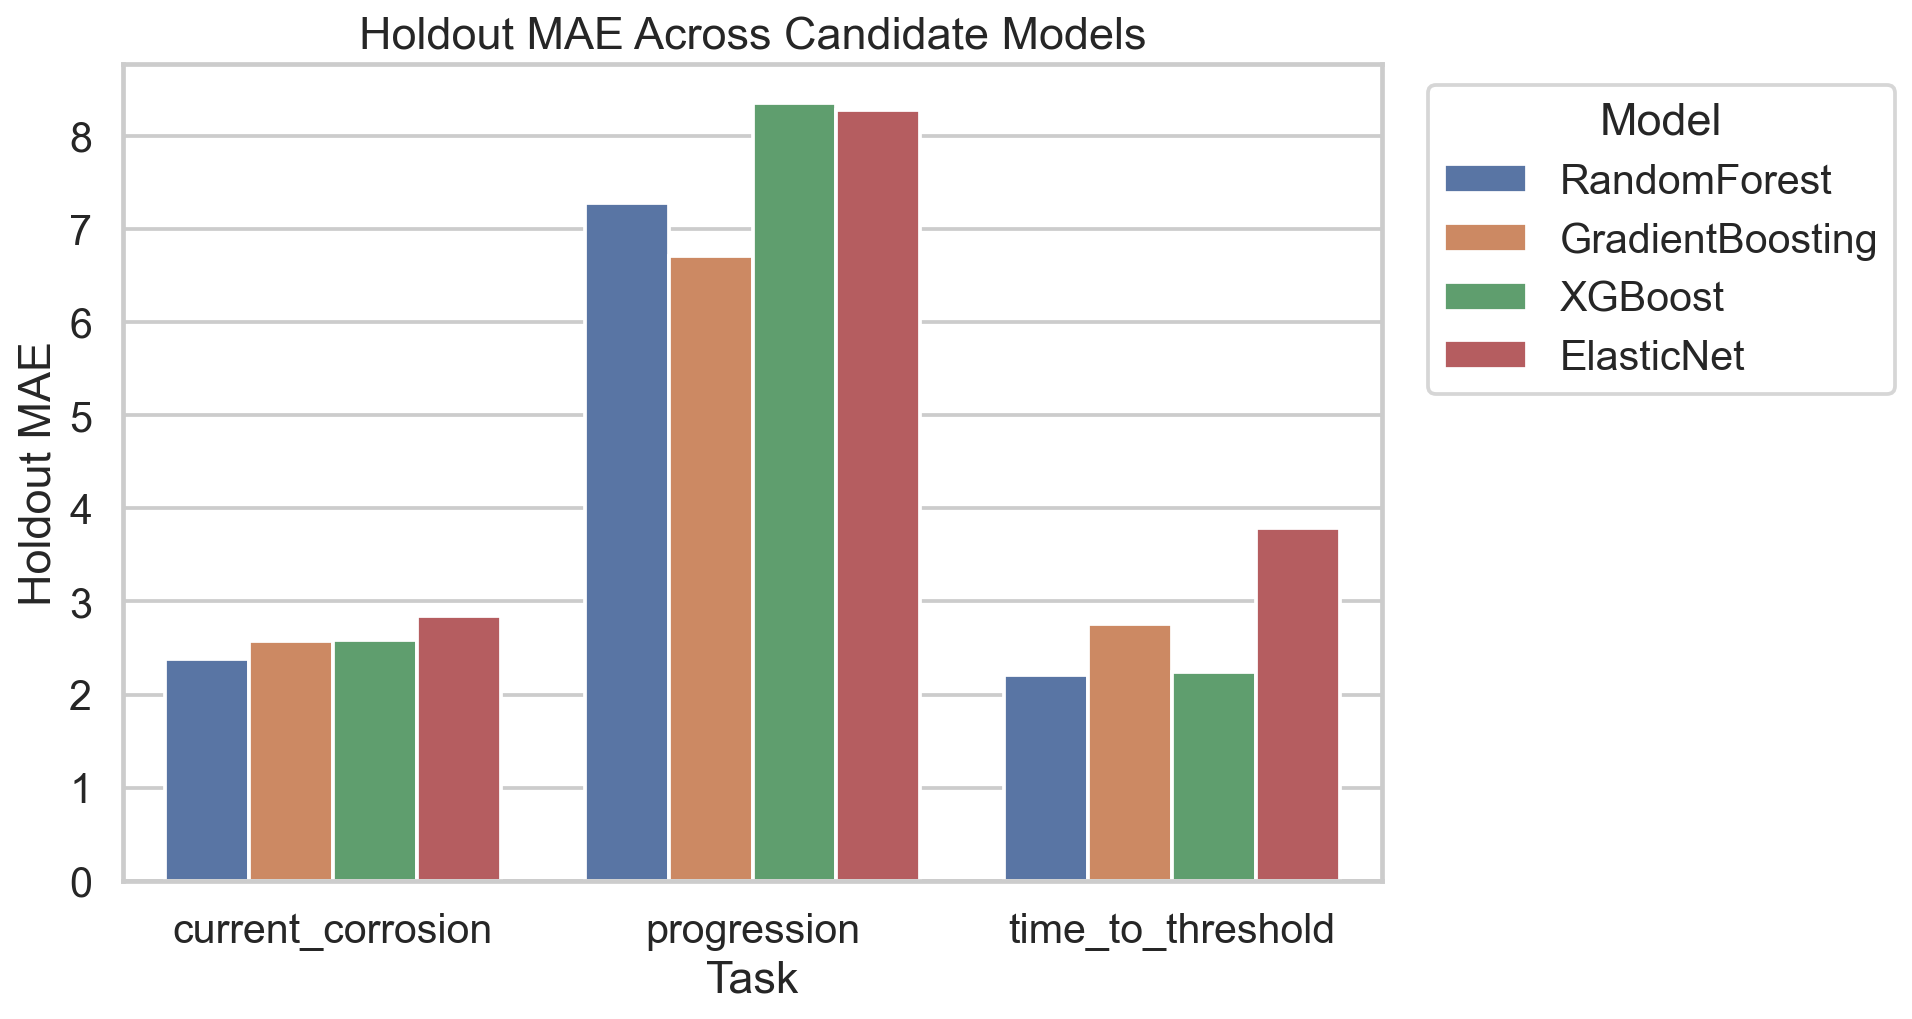
\includegraphics[width=0.86\textwidth]{reports/fig_holdout_mae_by_task.png}
\caption{Holdout MAE across candidate models for the three tasks. Current-corrosion prediction is the strongest task; progression is the weakest; time-to-threshold is numerically strong but conditional on a derived timing target and true current corrosion input.}
\label{fig:holdout_mae}
\end{figure}

\subsection{Strongly supported results}
\paragraph{1. The repository supports strong current visible-corrosion estimation.}
Task A achieves holdout MAE 2.3794 and \(R^2=0.8996\). The saved importance table and Figure~\ref{fig:current_importance} show that this performance is image-driven in a very specific way: it is dominated by the handcrafted rust-mask percentage.

\paragraph{2. The progression model is materially weaker and metadata-driven.}
Task B degrades to holdout MAE 6.7144 and \(R^2=0.5170\). The feature-importance table shows that week and cover dominate. This supports a narrower claim: the repository can regress corrosion level from metadata and time within the observed specimen families. It does not support a claim of learned corrosion dynamics from images.

\paragraph{3. The threshold-timing model is a proxy conditioned on current corrosion.}
Task C achieves holdout MAE 2.2114 weeks and \(R^2=0.7820\), but this number is conditional on true current corrosion being known and on the specimen belonging to the threshold-reaching subset.

\subsection{Weak, negative, and exploratory results}
\paragraph{Weak result: Task C is not a complete end-to-end pipeline metric.}
Because the time model uses the true \texttt{B\_Peak\_Rust\_Percentage\_[\%]} as an input feature during training and evaluation, its holdout score is not the performance of an image-to-threshold system. It is a conditional proxy benchmark.

\paragraph{Negative result: current reproducibility is broken.}
The training entry point currently fails on the present workbook with a \texttt{TypeError} inside \texttt{dataset\_summary()}, because \texttt{week} is all-missing after the identifier parser is applied to the current specimen-level \texttt{ID} column. Even if that failure were patched, the cached image-feature merge would still return all-\texttt{NaN} image features because the IDs no longer align.

\paragraph{Negative result: deployment claims in the repository are currently overstated.}
\texttt{load\_artifacts()} fails locally because \texttt{manifest.json} stores model paths under another user's home directory. The joblib files exist locally, but the current deployment code does not resolve them.

\paragraph{Exploratory result: threshold-reaching specimens cluster at late weeks.}

\begin{figure}[H]
\centering
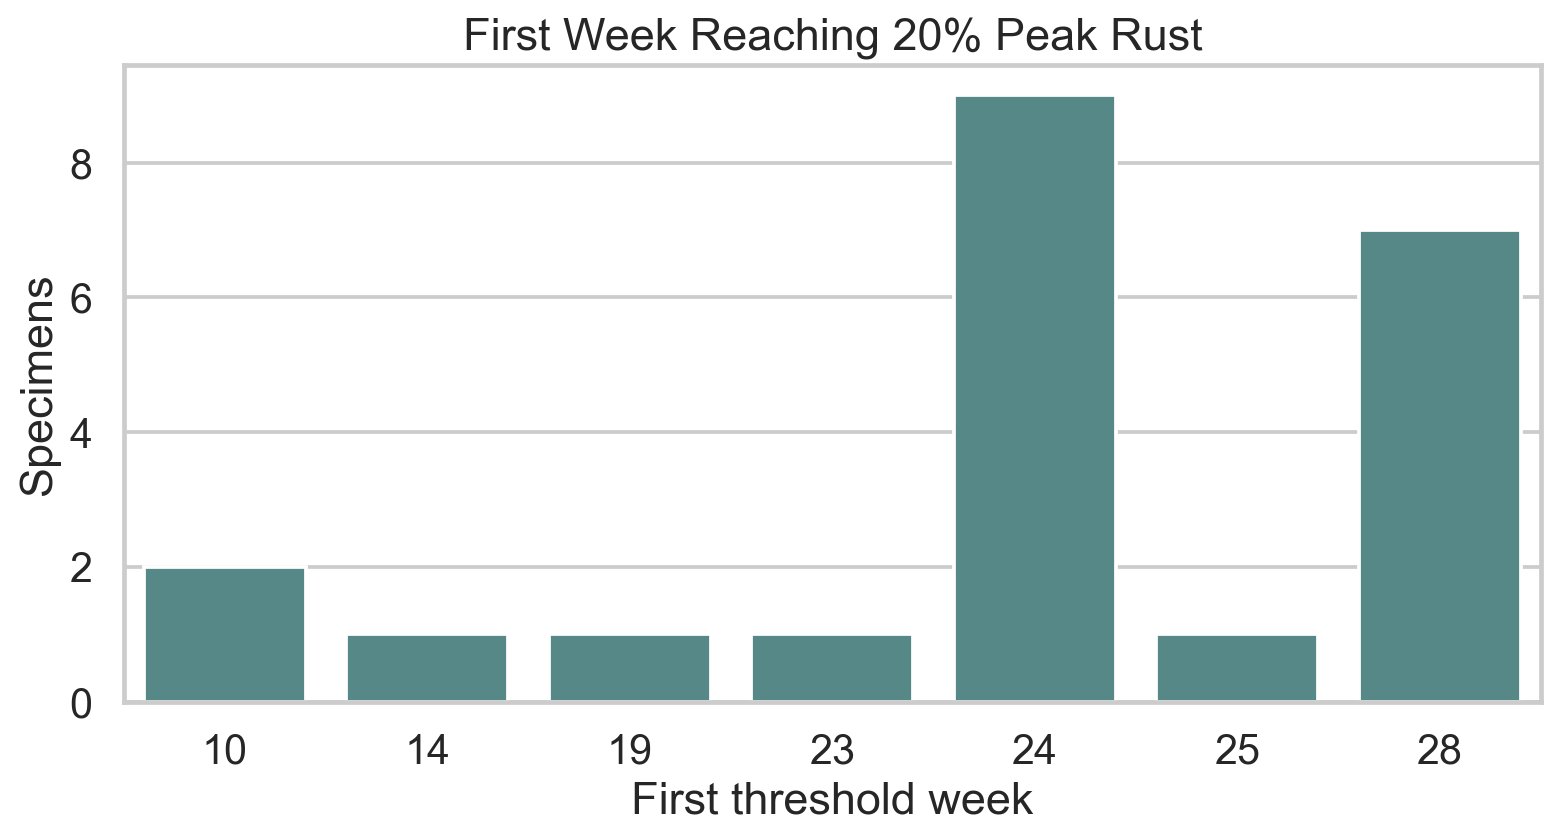
\includegraphics[width=0.74\textwidth]{reports/fig_threshold_event_weeks.png}
\caption{Distribution of the first observed week reaching the 20\% peak-rust threshold among the 22 threshold-reaching specimens. The proxy timing dataset is concentrated late in the campaign, especially at weeks 24 and 28.}
\label{fig:event_weeks}
\end{figure}

Figure~\ref{fig:event_weeks} shows that first threshold crossings are concentrated near weeks 24 and 28. This matters because the timing model is trained on a limited event-time distribution rather than on a broad range of failure regimes.

\subsection{What the results do \emph{not} justify claiming}
The saved outputs do not justify claiming that \texttt{main}:
\begin{itemize}
  \item predicts structural wire loss or ultimate load;
  \item performs direct image-to-RUL learning;
  \item has been validated on censored specimens for threshold timing;
  \item has been validated under treatment- or campaign-held-out transfer;
  \item reproduces the full strip-based thesis pipeline;
  \item is currently deployable without repair, despite what some repository prose implies.
\end{itemize}

\section{What the model can and cannot learn}

\subsection{What is directly visible and therefore learnable}
Task A can learn visible surface-rust patterns because it sees:
\begin{itemize}
  \item the global proportion of pixels within the documented rust RGB range;
  \item gross channel intensity differences associated with rust staining;
  \item brightness and saturation changes across the specimen surface.
\end{itemize}

This is why current-corrosion prediction is the strongest task in the repository.

\subsection{What may be indirectly inferable}
Through the metadata and family variables, the models may also infer:
\begin{itemize}
  \item specimen family or campaign-like grouping through \texttt{series};
  \item treatment condition through \texttt{Treatment};
  \item exposure stage through \texttt{week} and \texttt{Ageing\_Days};
  \item broad material design through cover thickness and mesh count.
\end{itemize}

These are useful for interpolation within the observed dataset, but they are also potential shortcut variables.

\subsection{What is hidden and not reliably recoverable here}
The implemented repository does not directly support reliable recovery of:
\begin{itemize}
  \item hidden internal corrosion or wire area loss from images;
  \item ultimate load from surface images;
  \item failure time under censoring;
  \item true campaign-robust remaining useful life;
  \item physically constrained monotonic degradation trajectories.
\end{itemize}

\subsection{Why some targets are easier than others}
The difficulty ranking in the saved outputs is scientifically coherent:
\begin{itemize}
  \item \textbf{Current corrosion} is easiest because the handcrafted features directly measure visible rust-like pixels.
  \item \textbf{Progression} is harder because the model sees no image and must infer corrosion from metadata plus week.
  \item \textbf{Time to threshold} appears stronger numerically than progression because it is trained on a subset of threshold-reaching specimens and receives the true current corrosion label as an input.
\end{itemize}

\subsection{Why metadata may outperform image features in some tasks}
In Task B and Task C, metadata dominate because the task definitions themselves rely on temporal and specimen context. In this repository, metadata do not merely supplement the images; in two of the three tasks they are the entire model input or the majority of the explanatory signal.

\section{Traceability to original thesis and documentation}

\subsection{What the documentation says}
The local thesis and conference paper describe a broader workflow with:
\begin{itemize}
  \item GIMP-based cropping and white-balance preprocessing;
  \item BIMP batch processing to a standard PNG format;
  \item MATLAB RGB-threshold segmentation;
  \item strip-wise analysis along specimen length;
  \item corrosion categorization into low, medium, and high evidence;
  \item in the conference paper, a ResNet-50 classifier trained on those categories.
\end{itemize}

\subsection{What \texttt{main} actually reproduces}

\begin{table}[H]
\centering
\small
\begin{tabularx}{\textwidth}{p{0.29\textwidth} p{0.29\textwidth} Y}
\toprule
\textbf{Documented method} & \textbf{What \texttt{main} reproduces} & \textbf{Expected consequence of the mismatch} \\
\midrule
GIMP/BIMP preprocessing with white balance, crop, and batch export & Not executed in code; assumed upstream in the existing PNG set & If current PNGs drift from the documented preprocessing, feature behavior can shift. \\
MATLAB RGB-threshold corrosion extraction & Partially reproduced only through three fixed RGB threshold masks and global color statistics & The code preserves the threshold logic but not the full segmentation workflow. \\
Strip-wise peak-corrosion computation along specimen length & Not reproduced in feature extraction & The current image features are global, whereas the target label originates from a peak quantity. \\
Three-class corrosion categorization at \(<1\%\), \(1\%-<20\%\), and \(\geq20\%\) & Reused in current-corrosion class labeling and in threshold logic & The threshold semantics are preserved, but the learned task is regression, not classification. \\
ResNet-50 transfer learning on corrosion categories (conference paper) & Not reproduced in \texttt{main}; this repository uses classical regressors on handcrafted features & The saved results are not directly comparable to the conference model architecture or accuracy claims. \\
Scientific-solution text claiming validated local deployment & Not currently true in code because the manifest paths are stale & User-facing documentation overstates present deployability. \\
\bottomrule
\end{tabularx}
\caption{Comparison between the documented original workflow and the executable \texttt{main} implementation.}
\label{tab:traceability}
\end{table}

\subsection{What could not be recovered exactly}
The repository does not contain the original MATLAB strip-analysis code, the full BIMP configuration, or a documented rule for reconstructing the \texttt{NaCl\%} feature from the current raw workbook. Therefore the exact preprocessing and feature-assembly path that produced the historical saved models cannot be fully recovered from the current raw files alone.

\section{Limitations}

The main limitations are specific to the actual repository state:
\begin{enumerate}
  \item \textbf{Three tasks, three different scientific meanings.} The repository is not one coherent image-to-life model. It mixes visible-corrosion regression, metadata-conditioned interpolation, and derived threshold timing.
  \item \textbf{Sparse structural endpoints.} Wire loss and ultimate load are terminal specimen-level labels only and are not modeled.
  \item \textbf{Proxy timing target.} The time-to-threshold model excludes 26 censored specimens and uses true current corrosion as an input.
  \item \textbf{No end-to-end threshold evaluation.} The saved outputs do not measure chained performance from image \(\rightarrow\) current corrosion prediction \(\rightarrow\) time-to-threshold prediction.
  \item \textbf{Perfect temporal redundancy.} \texttt{Ageing Days} and \texttt{week} are redundant in the current workbook.
  \item \textbf{Handcrafted-feature tautology risk.} The dominant current-corrosion feature is a rust-threshold area closely aligned with the documented corrosion labeling logic.
  \item \textbf{No strict transfer splits.} The repository does not evaluate leave-one-treatment-out, leave-one-series-out, or campaign-held-out robustness.
  \item \textbf{Aggregate outputs only.} No holdout predictions, residual plots, or saved split memberships are available for deeper error auditing.
  \item \textbf{Broken current reproducibility.} The live training code no longer matches the present raw workbook, the current cache no longer merges, and the live API loader fails on stale absolute paths.
  \item \textbf{External validity remains narrow.} The results are tied to one experimental repository, one image-preprocessing lineage, and a handcrafted visual threshold strategy.
\end{enumerate}

\section{Future work}

The next steps that logically follow from the actual repository state are repair and disambiguation, not generic model escalation:
\begin{enumerate}
  \item \textbf{Repair the data contract.} Update the loader to parse row-level IDs from \texttt{Sample Name}, rename or map \texttt{Ageing Days} to \texttt{Ageing\_Days}, and document how \texttt{NaCl\%} should be reconstructed.
  \item \textbf{Make artifact loading relative-path based.} The current manifest prevents local deployment even though the model files exist.
  \item \textbf{Persist split membership and per-row predictions.} Without them, the current results cannot be audited at specimen level.
  \item \textbf{Decide whether the project is primarily image-based or metadata-based.} In \texttt{main}, Tasks B and C are not image-driven; that should be an explicit design choice rather than an accidental side effect.
  \item \textbf{If threshold timing is the real goal, evaluate end-to-end chaining.} Measure the full image \(\rightarrow\) current corrosion \(\rightarrow\) time-to-threshold path rather than only the conditional time model.
  \item \textbf{If thesis reproducibility matters, restore strip-wise logic.} The current global image features are not the documented strip-analysis pipeline.
  \item \textbf{If hidden structural degradation matters, design a new supervision strategy.} The current labels are too sparse and too terminal for direct structural modeling.
  \item \textbf{Remove or constrain redundant temporal inputs.} The progression and timing endpoints should not accept inconsistent \texttt{week}/\texttt{ageing\_days} combinations.
\end{enumerate}

\appendix

\section{Meeting-defense questions and concise evidence-based answers}

\paragraph{Why not direct RUL?}
Because no raw RUL label exists, no survival model is implemented, and the time target in \texttt{main} is a derived threshold-crossing proxy created from the corrosion label and week.

\paragraph{Why these split strategies?}
Because each specimen is observed repeatedly over time. Grouping by specimen is the minimum required control against repeated-measures leakage.

\paragraph{Why did robustness drop from current corrosion to progression?}
The strongest current model uses image features dominated by rust-mask percentage, which directly measures visible corrosion evidence. The progression model has no image input and relies mostly on week and cover, so it solves a less direct problem.

\paragraph{Why can visible corrosion be predicted better than structural degradation?}
Visible corrosion is present in the image and in dense labels. Structural damage variables are hidden and only sparsely observed at specimen endpoints.

\paragraph{How much of the signal comes from metadata?}
It depends on the task. For current corrosion, the dominant saved feature is the image-derived rust-mask percentage. For progression and timing, metadata and current corrosion carry nearly all of the usable signal.

\paragraph{What are the highest-risk assumptions?}
The largest risks are the broken ID mapping, the missing documented raw \texttt{NaCl\%} field, the use of holdout MAE for model selection, the assumption that the current PNGs still reflect thesis-style preprocessing, and the use of true current corrosion in the timing benchmark.

\paragraph{Could preprocessing mismatch explain part of the gap between documentation and code?}
Yes. The thesis and conference documents emphasize GIMP/BIMP preprocessing and strip-based MATLAB analysis, but \texttt{main} uses compact global descriptors and assumes the PNG set is already normalized appropriately.

\paragraph{Which features are most interpretable?}
The most interpretable features are the handcrafted mask percentages, especially \texttt{img\_rust\_mask\_pct}, and the metadata fields such as week, cover, and treatment. These are far more interpretable than latent deep features, but they also make tautology and shortcut risks easier to see.

\paragraph{What exactly is meant by each major output?}
\begin{itemize}
  \item \textbf{current corrosion}: current peak-rust percentage for the same observation.
  \item \textbf{progression curve}: a metadata-conditioned sweep of predicted peak rust over week, not a sequence forecast with memory.
  \item \textbf{predicted threshold week from progression}: first week on that swept curve whose predicted rust exceeds the threshold.
  \item \textbf{time to threshold}: a separate regression model's predicted remaining weeks, conditioned on current corrosion and metadata.
\end{itemize}

\paragraph{Are the two threshold outputs guaranteed to agree?}
No. The repository contains two separate threshold mechanisms: progression-curve crossing and the dedicated time-to-threshold regressor. No consistency check or calibration between them is saved.

\paragraph{Can the API be used as-is now?}
No. The current \texttt{manifest.json} points to model files on another machine, so \texttt{load\_artifacts()} fails locally unless the paths are repaired.

\end{document}
